\graphicspath{{chapters/6.Chapter_4/figures}}
 
\begin{savequote}[75mm]
``All models are wrong, but some are useful''
\qauthor{- George E.P. Box & Draper: \textit{Empirical model-building and response surfaces, 1987}}
\end{savequote}



\chapter{Endosymbiont Metabolic Analysis}

http://www.sciencedirect.com/science/article/pii/S0888754312000250 - see this for analysis to copy \citep{Xie2012}

What is the endosymbiont doing? - metabolic map

How does it differ between day and night? - differential expression

What does it need?

What is it secreting? (control against NC64A chlorella signal peptides - are we missing anything obvious in transcriptome endosymbiont bin)



UBLAST and cut-off for KO annotation, IPATH2.0 for maps  \citep{Wisecaver2014}

Also of interest is the activity of fatty acid and amino acid biosynthesis in the endosymbiont.  This is because
all well studied examples of primary of secondary plastids that have lost photosynthetic activity appear to maintain 
essential roles in these and other areas of host metabolism.
In all well-studied cases to date, the plastid itself is retained, as it is known to be the site of essential biochemical processes unrelated to photosynthesis, including fatty acid and amino acid biosynthesis (Waller and McFadden 2005; Barbrook et al. 2006; Mazumdar et al. 2006). \citep{Donaher2009}

Additionally the comparison of photosynthetic \textit{Symbodinium} within their cindarian hosts in both autotrophic and mixotrophic conditions
is of interest \citep{Xiang2015}

Genes indeitnfied in paramecium tetaurelia involve din autogamy, reciliation and exocytosis respectively \citep{Arnaiz2010}
Interestingly highly differentially expressed genes appear to have a lower rate of gene loss \citep{Arnaiz2010}

Diffeq - single cell - technical noise important - must be quantifeid so it can be incorporated into 

Low amount of RNA in single cell presents a major difficulity leading to unavoiable technicla noise \citep{Brennecke2013}

Depth


Unfortunately no ERCC because reasons
http://www.nature.com/nmeth/journal/v10/n11/extref/nmeth.2645-S2.pdf




mycosporina amino acids - shikimate pathway - protect agains UVR \citep{Sommaruga2009} (Shick and dunlap 2002)
chlorella made MAA found in cilliates sonntag2007 
Negative in p bursaria chlorella thoufgh summerer2009


PSI-BLAST is more sensitive to distance evolutionary relationships that standard blast

\subsection{Metacyc vs KEGG}

More pathways in metacyc - closer to real  
biocyc and kegg 


\subsection{Metabolomics}

NMR was the traditional method - less sample preparation, rapid, nondestructive, high-throughput, robust

LC - good for polar/apolar but bad frag, ion supression and small/very polar need special column
GC - suited for apolar and volatiles - universal databank but needs high sample prep, derivatizatrion of polar and lots of frag





gT



\section{Aims}

Identify 



\section{Methods}



\subsection{Mteabolomics}



\subsection{Untargeted Metabolomic Profiling} 

A global metabolomic profile was profiled using 
GC/QTOF and LC/QTOF (with positive and negative polarity).

LC-QTOF was conducted using


abd were charged using dual electronspray ionisation (ESI), one run
using a negative polarity and the other positive. 



\(3.5\mu m\), \(2.1 \times 150mm\) Eclipse Plus C18 (Agilent) 





In order to determine differential presence of globally detected metabolites
unpaired Welch's \textit{t}-tests were conducted comparing the 5 day samples to the 5
night samples. Welch's tests were used as they don't assume equal sample sizes or variances
between the two groups\citep{Welch1947}\footnote{
    \(t' = \frac{\mu_1 - \mu_2}{\sqrt{\frac{s^2_1}{n_1} + {s^2_2}{n_2}}}\)
    with degrees of freedom determined via the Welch-Satterwaite-equation:
    \(df = \frac{(\frac{s^2_1}{n_1} + \frac{s^2_2}{n_2})^2}{\frac{(\frac{s^2_1}{n_1})^2}{n_1 - 1} + \frac{(\frac{s^2_2}{n_2})^2}{n_2 - 1}}\)
    \citep{Ruxton2006}
}

P-values from this were corrected 
for multiple comparisons using false discovery rates (FDR).  FDR is a
less conservative correction than, the classic family-wise error rate correction,
Bonferroni adjustment\footnote{
    P-value threshold \(\alpha\) is adjusted relative to the number of comparisons (n). 
Specfically, significance is determined as a P-value \(\leq \frac{\alpha}{n}\).} but
allow maintenance of a greater proportion of statistical power with a 
slightly evelated risk of Type-I errors. 






\subsection{Targeted Amino Acid Profiling}

A targeted quantitative analysis of amino acid concentration between day
and night was conducted
using targeted MS/MS via LC-QQQ using an Agilent 1200 HPLC stack and a 
Agilent 6410 enhanced sensitivity  
quadrupole (QQQ) mass spectrometer. 





\subsubsection{Qualitative MS}

Agilent 6520 accurate mass quadrupole time of flight (Q-TOF) 
with Agilent 1200 series HPLC stack

Agilent data acquisition software was used to parse the raw data
before conversion to the open mzXML format. 

Peaks were identified in each sample individually using XCMS xmcsSet
function and a matched filter with a step size of 0.01, a signal:noise threshold
of 10 and 2 steps 

extracted ion base peak chromatograms
%what is this?  


Identified peaks are then grouped across samples based on the m/z ratios
alignment
smoothed peak distribtuions 
samples only detected in some replicate of given class i.e. day or night 
are rejected at this stage.


Aligned and matched peaks were then used to evaluate changes in retention time during
chromatography between samples.  Calculated drift correlations were then used to
improve the alignment and grouping of peaks.




\subsubsection{GCMS}

GCMS data was analysed using metaMS.

Pseudospectrum approach instead of peak alignments etc due to the difficulties
aligning data of this type relative to LCMS.

Peak picking followed by pseudospectra determination.
Identification and elemeiaton of artefacts and then annotation
against a standards database. 

Rather than individual peaks - a pseudospecvtrum is used.
This is a set of m/z values with a peak at the same rentetion time.
In GC the overalp is smaller than in LC due tot he narrower peaks therefore
retention times are harder to match leading to separate mass spectra. 

NIST library has fragmentation patterns.

Spectra are easier to interepr due to adducts - 



Comparison of pseudospectra is done via a weighted dot product



Finally unannotated patterns repeatedly occur in different 


http://www.bioconductor.org/packages/3.3/bioc/vignettes/metaMS/inst/doc/runGC.pdf





\subsection{Quantitative MS}

\subsubsection{Amino acids}

MRM for more accurate analysis 

Agilent 6410 enhanced sensitivity triple quadrupole (QQQ) 
with Agilent 1200 series HPLC stack

\subsubsection{Carbohydrates}


\subsection{Annotation}

Sequences were annotated using the results from BLAST, InterproScan
and BLAST2GO mapping used to identify \textit{M. reisseri} transporters
in the previous chapter. 



\subsection{Mapping}


\begin{figure}
	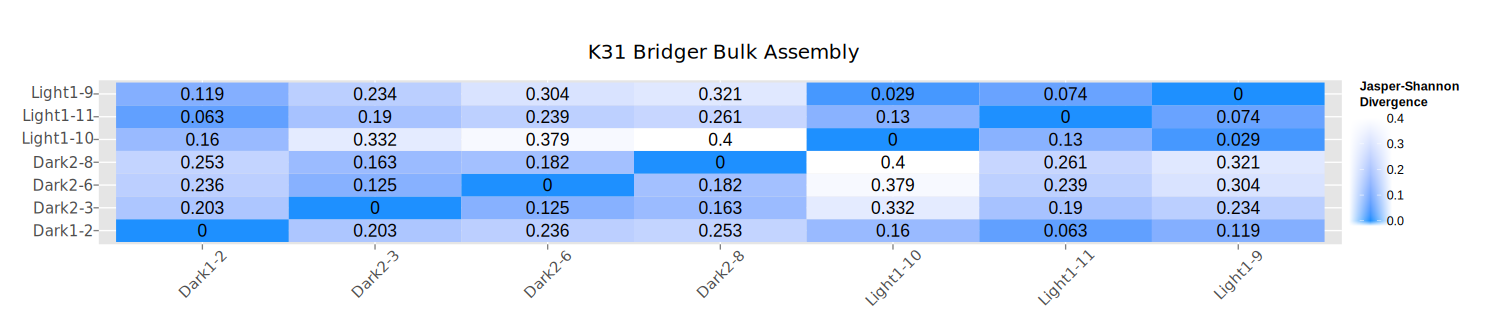
\includegraphics{bridger_bulk_only_sct_kallisto_mapping_jsd.pdf}[width=\textwidth]
	\caption{SCT sample-wise similarities - entire libraries post trimming
		no error correction or normalisation mapped to a Bridger transcriptome 
		assembly of an error corrected, digitally normalised Bulk Assembly.  
		This was conducted to check whether similarities between samples
		were being biased by something?}
	\label{fig:bridger_bulk_heatmap}
\end{figure}


\section{Results}


\subsection{Metabolomics} 

\subsubsection{Targeted QQQ LCMS}

\begin{figure}
    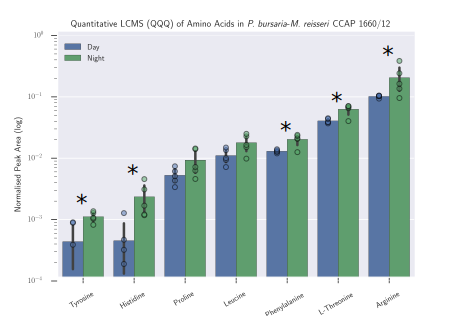
\includegraphics[width=\textwidth]{AA_LCMS.pdf}
    \caption{Normalised LCMS Peak Areas - 
        Calibration was conducted using Day1 and Night1 samples at two titrations, as well as Asn-Gln-Tryptamine and Sigma AA mixes
    Calibration and quantitative analysis failed for the following amino acids: 
Glutamic Acid, Tryptamine, Asparagine, Trpytophan, Isoleucine, Methionine, Valine, Serine, Glutamate, Glutamine, Aspartic acid, Cystein or Lysine.
Significant concentration differences between day and night (as determined via Welch's `\textit{t}' are indicated by an astrerisk.}
    \label{fig:aa_lcms}
\end{figure}

\subsubsection{Carbohydrate GCMS}


\subsubsection{Qualitative QTOF LCMS Profiles}


\section{Discussion}

\subsection{Limits of metabolomics analysis}

A more intelligent hypothesis testing than corrected unequal variance 't'-test
could be used such as Kurschke's Bayesian BEST algorithm \citep{Kruschke2013}.
This also has the advantage of a Bayesian inference which can be 
made robust to multiple comparisons without need for extensive correction
procedures by using standard multi-level approaches \citep{Gelman2009}.




